\chapter{Overview of Tool}\label{sec:swinstruct}
This chapter describes the different abilities in the program and how they are
used.

\section{Interface}
The interface of the program is based on two parts.  First, a command line
interface (CLI) where input and output is handled.  Second, a graphical
presentation of images, using the matplotlib library in Python which allows for
plotting several images in the same area.

Eg. the CLI simply looks like the following snippet below.  While the graphical
display of images is shown in figure \ref{fig:gui_display}.
The CLI is controlled through very specificly formatted commands and responses
from queries by the system.
\lstinputlisting{chapters/appendices/menu.txt}
\begin{figure}[h]
	\center
	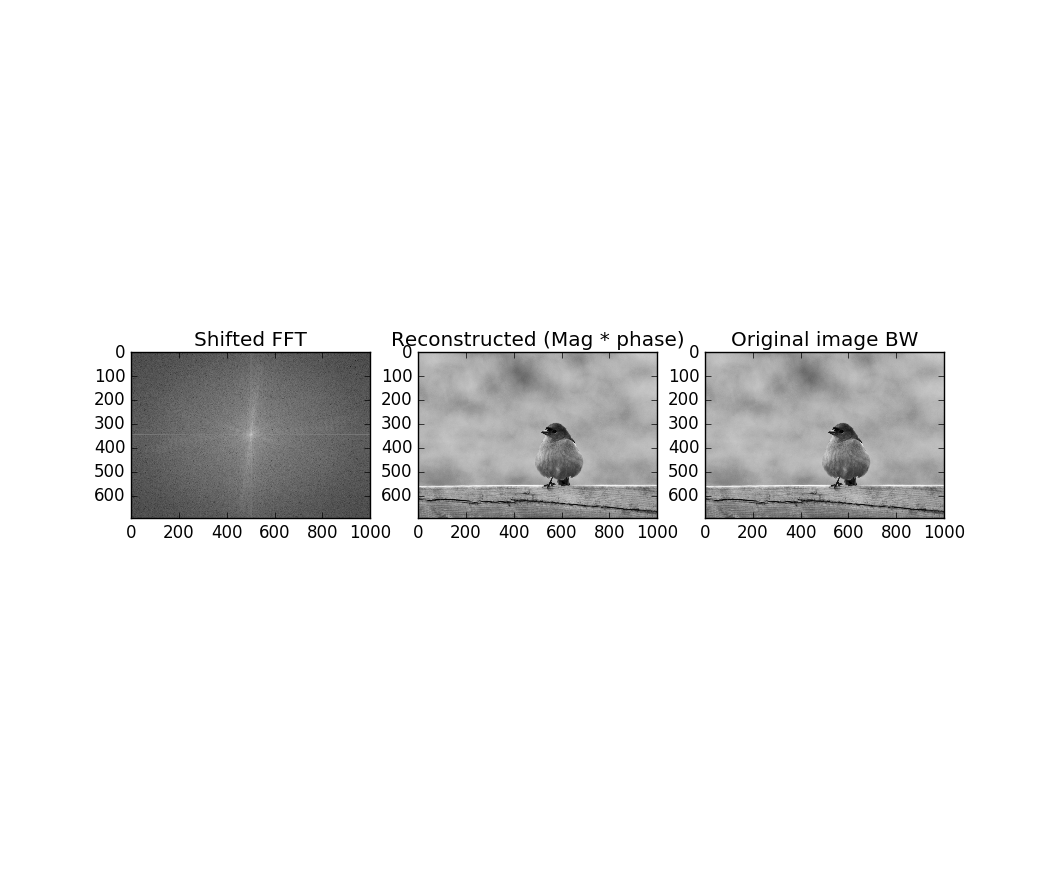
\includegraphics[width={1\linewidth},trim={50px 235px 50px 230px},clip]{pics/gui_display}
	\caption{Graphical visualisation of images}\label{fig:gui_display}
\end{figure}



\section{Filter Filter}


\begin{multicols}{2}
\begin{enumerate}
	\item 
\end{enumerate}
\end{multicols}

\section{}


\section{Comparison}
THe comparison regime installed in this application is based on the evaluation
of histogram data of the image which is being compared.  The comparison metrics
being generated is the following.
\begin{multicols}{3}
\begin{enumerate}
	\item Manhattan Distance
	\item Eucledian Distance
	\item Cosine Distance
	\item Match Distance
	\item Root Mean Squared Error
\end{enumerate}
\end{multicols}

\paragraph{Manhattan Distance}
Manhattan distance is a commonly used metric for measuring the difference
between two values.
\begin{align}
	D_{manhattan} &= \Sigma^{M,N}_{x,y} | H_{a}(x,y) - H_{b}(x,y) |
\end{align}

\paragraph{Eucledian Distance}
Eucleadian is quite similar to Manhattan distance, but the result of Manhattan
is squared.
\begin{align}
	D_{euclid} &= \Sigma^{M,N}_{x,y} |H_a(x,y) - H_b(x,y)|^2 
\end{align}

\paragraph{Cosine Distance}
\begin{align}
	D_{cosine} &= \Sigma^{M,N}_{x,y}  H_a(x,y) * H_b(x,y)
\end{align}

\paragraph{Match Distance}
\begin{align}
	D_{match} & = \Sigma^{M,N}_{x,y} |H_a(x,y) - H_b(x,y)|
\end{align}

\paragraph{ Distance}
%\begin{align}
%	D_{} & = \Sigma^{}_{} 
%\end{align}

\section{Additional functionality}
In addition to the previously mentioned abilities in the program there are
several extra features built in to the program.  Among others are that the
database is arbitrary and can take any image and perform the actions on it, 
given that it's either "JPEG", "BMP", "TIFF" or "PNG" formatted.

The images can be saved, either upon exiting the software or explicitly telling
the program to save the selected images.  This will save the image as a "JPEG"
formatted image in the "./outdir" and a text file containg the metric data
belonging to the image.

